% ============================================================
% FINAL PROJECT REPORT - ENGLISH VERSION
% Project 07: Document-Level OCR with Post-OCR Correction
% Course: CSC15012 - Applications of NLP in Industry
% Student: Le Dinh Minh Quan - 23127460 - 23CNTThuc
% ============================================================
\documentclass[12pt,a4paper]{article}

\usepackage[utf8]{inputenc}
\usepackage{geometry}
\geometry{left=2.3cm, right=2.3cm, top=2.5cm, bottom=2.5cm}
\usepackage{setspace}
\setstretch{1.25}
\usepackage{graphicx}
\usepackage{float}
\usepackage{booktabs}
\usepackage{longtable}
\usepackage{tabularx}
\usepackage{array}
\usepackage{hyperref}
\hypersetup{colorlinks=true, linkcolor=blue, urlcolor=blue, citecolor=blue, breaklinks=true}
\usepackage{xurl}
\usepackage{seqsplit}
\usepackage{listings}
\usepackage{xcolor}
\usepackage{amsmath}
\usepackage{caption}
\usepackage{subcaption}
\usepackage{enumitem}
\usepackage{fancyhdr}
\usepackage{tikz}
\usetikzlibrary{shapes.geometric, arrows.meta, positioning, fit, backgrounds, shadows}

% --- Make long inline code / paths break gracefully ---
\sloppy
\tolerance=2000
\emergencystretch=3em
\hbadness=10000
\setlength{\parskip}{0.15em}

% Helper for breakable monospaced paths
\newcommand{\bpath}[1]{\seqsplit{#1}}
\newcommand{\btt}[1]{\texttt{\seqsplit{#1}}}

% New column type for tabularx: left-aligned and ragged-right with breaking
\newcolumntype{L}{>{\raggedright\arraybackslash}X}

\lstset{
  basicstyle=\ttfamily\small,
  breaklines=true,
  frame=single,
  backgroundcolor=\color{gray!10},
  keywordstyle=\color{blue},
  commentstyle=\color{green!60!black},
  stringstyle=\color{red!70!black},
  showstringspaces=false,
  tabsize=2
}

\pagestyle{fancy}
\fancyhf{}
\fancyhead[L]{\small CSC15012 -- Final Project Report}
\fancyhead[R]{\small Le Dinh Minh Quan -- 23127460}
\fancyfoot[C]{\thepage}

% ============================================================
\begin{document}

% --- TITLE PAGE ---
\begin{titlepage}
\centering
\vspace*{0.5cm}

% HCMUS LOGO: upload logo_hcmus.png to Overleaf and uncomment the next line
\IfFileExists{logo_hcmus.png}{\includegraphics[width=3.5cm]{logo_hcmus.png}\\[0.5cm]}{}

{\large \textbf{VIETNAM NATIONAL UNIVERSITY HO CHI MINH CITY}}\\[0.3cm]
{\Large \textbf{UNIVERSITY OF SCIENCE}}\\[0.3cm]
{\large Faculty of Information Technology}\\[1.5cm]

{\LARGE \textbf{FINAL PROJECT REPORT}}\\[0.5cm]
{\large Course: \textbf{CSC15012 -- Applications of Natural Language\\ Processing in Industry}}\\[1.5cm]

{\Large \textbf{Project 07:}}\\[0.3cm]
{\Large \textbf{Document-Level OCR with Post-OCR Correction}}\\[0.3cm]
{\large A Layout-Aware OCR Pipeline with a Trainable ByT5 Corrector and an Agentic Orchestrator}\\[2cm]

\begin{tabular}{ll}
\textbf{Student:} & Le Dinh Minh Quan \\
\textbf{Student ID:} & 23127460 \\
\textbf{Class:} & 23CNTThuc \\
\end{tabular}

\vfill
{\large Ho Chi Minh City, 2026}
\end{titlepage}

\tableofcontents
\newpage

% ============================================================
\section{Introduction}
% ============================================================

Real-world documents arrive as page images and scanned or born-digital PDFs. A single \emph{flat} OCR pass over a full page produces an \textbf{unordered, error-riddled text dump}: the reading order is wrong on multi-column pages, there is no block typing (title vs.\ table vs.\ footer), and the characters themselves are garbled (\texttt{rn$\rightarrow$m}, \texttt{0$\leftrightarrow$O}, \texttt{1$\leftrightarrow$l}, merged and split words). Clean, structured text is the upstream feed for search, retrieval-augmented generation (RAG), analytics, compliance, and data entry, so this raw dump is rarely usable as-is.

This project implements a complete \textbf{Document-Level OCR System} end-to-end. It turns a document image / PDF into clean, \textbf{structured, reading-order-correct} text (Markdown + typed JSON blocks + plain text), with:
\begin{itemize}
  \item An OCR front-end plus layout analysis and reading-order recovery (pretrained / algorithmic) for \emph{structure};
  \item A \textbf{trainable post-OCR correction model} (a character-level \texttt{google/byt5-small} seq2seq) that measurably lowers Character/Word Error Rate (CER/WER) on top of \emph{any} OCR engine -- the one trained differentiator;
  \item A \textbf{deterministic agentic pipeline} (a finite-state machine with four explicit decision points + an optional, validated LLM brain) that orchestrates the whole document $\rightarrow$ structured-text flow;
  \item Production deployment as a FastAPI REST API, a Gradio demo UI, a CLI, and a Docker image, plus a one-button Colab H100 autopilot that trains, evaluates, and self-grades.
\end{itemize}

\textbf{Project Resources (public):}
\begin{itemize}\setlength\itemsep{0.15em}
  \item \textbf{GitHub repository (source code):} \url{https://github.com/ledinhminhquan/07_Document_Level_OCR}
  \item \textbf{Trainable model:} \texttt{google/byt5-small} (Apache-2.0); T4 fallback \texttt{google-t5/t5-small} (Apache-2.0)
  \item \textbf{Primary real corpus:} \texttt{PleIAs/Post-OCR-Correction} (config \texttt{english}, CC0-1.0)
  \item \textbf{Colab H100 autopilot notebook:} \texttt{notebooks/DocOCR\_Colab\_Training\_H100\_AUTOPILOT.ipynb} (+ \texttt{COLAB\_GUIDE.md})
\end{itemize}

\noindent\textit{Deployment status.} The system is \textbf{deployable} (FastAPI + Gradio + Docker + a Hugging Face Space packaging + a one-button Colab autopilot). The numbers reported here are \textbf{verified offline} on a synthetic OCR-noise spine (with the real PleIAs slice), and the full Colab H100 run produces the complete metric tables; there is no public live demo URL.

% ============================================================
\section{Business Problem Definition}
% ============================================================

\subsection{Context and Motivation}

Organizations sit on large volumes of documents -- archives, invoices, forms, reports, scanned correspondence -- that need to become machine-readable. The challenges with a naive OCR pass are:
\begin{itemize}
  \item \textbf{Accuracy}: char-level OCR garble (\texttt{rn$\rightarrow$m}, \texttt{0$\leftrightarrow$O}, \texttt{1$\leftrightarrow$l}, merge/split) corrupts every downstream consumer.
  \item \textbf{Structure}: a flat dump has no typed blocks and no reading order, so RAG and table extraction cannot use it.
  \item \textbf{Cost}: high-accuracy commercial OCR engines are expensive; born-digital pages should not pay the OCR cost at all.
\end{itemize}

The product thesis is three levers: \textbf{(1) accuracy} -- a trained corrector lowers errors; \textbf{(2) structure} -- Markdown/JSON with typed, ordered blocks unlocks downstream use; \textbf{(3) engine-agnostic uplift} -- the corrector improves \emph{any} OCR backend, so it compounds with cheap CPU OCR (Tesseract) instead of requiring an expensive engine.

\subsection{Target Users and Stakeholders}

\begin{itemize}
  \item \textbf{Archivists \& libraries}: digitize scanned collections into searchable, reading-order-correct, typed text.
  \item \textbf{Businesses digitizing records}: convert invoices, forms, and reports to machine-readable data; born-digital pages skip OCR (D2) to cut cost per page.
  \item \textbf{Accessibility users}: reading-order-correct structured text is far more usable with screen readers than a raw dump.
  \item \textbf{Developers \& researchers}: an easy-to-integrate REST API plus a reproducible corpus and reported CER for auditable results.
\end{itemize}

\subsection{Problem Statement}

Given a document image or PDF, the system must:
\begin{enumerate}
  \item \textbf{Extract structure}: detect regions, type them (heading / paragraph / list / header-footer / blank), and recover the correct reading order (multi-column aware).
  \item \textbf{Improve text quality}: lower CER/WER with a trained post-OCR corrector, \emph{without making text worse}.
  \item \textbf{Emit a lossless, traceable result}: Markdown (human view) + JSON \texttt{blocks[]} (machine view) + plain text, with per-region confidence, \texttt{needs\_review} flags, and a full decision/audit manifest.
\end{enumerate}

\subsection{Why NLP is Required}

OCR errors are not random: they are context-dependent character/word events (confusable glyphs, merges, splits). A rule- or dictionary-only approach has no model of context and cannot cleanly fix merge/split errors or real-word substitutions. A learned \emph{sequence-to-sequence} corrector, trained on the actual OCR error distribution, is required to lower CER/WER reliably -- this is the NLP core of the project.

\subsection{Success Metrics}

\begin{table}[H]
\centering
\caption{System success metrics. The headline technical KPI is CER/WER \emph{reduction} versus the raw-OCR identity baseline, gated by a per-example safety check.}
\begin{tabular}{lll}
\toprule
\textbf{Type} & \textbf{Metric} & \textbf{Target} \\
\midrule
Business  & Manual-review reduction (\% pages auto-accepted) & Maximize \\
Business  & Structure fidelity (\% blocks typed + ordered) & High \\
Business  & Cost per page (born-digital skips OCR via D2) & Low (CPU default) \\
Technical & CER reduction (primary) vs.\ identity floor 0.088 & Clearly $>$0 \\
Technical & WER reduction vs.\ identity floor 0.49 & Clearly $>$0 \\
Technical & Safety gate (\% degraded $\ll$ \% improved) & Hard go/no-go \\
Technical & Latency, born-digital page (D2 skip) & $\sim$200\,ms \\
\bottomrule
\end{tabular}
\end{table}

The safety gate is decisive: a corrector that ``fixes'' 40\% of regions but breaks 30\% is near-useless, so we require \textbf{degraded $\ll$ improved} as an explicit pass/fail condition, reported alongside the headline reduction.

% ============================================================
\section{Development Infrastructure \& Tooling}
% ============================================================

\subsection{Repository Structure}

The project follows a production-ready Python package structure (\texttt{src/dococr/}), mirroring the public GitHub repository \url{https://github.com/ledinhminhquan/07_Document_Level_OCR} one-to-one. Heavy dependencies (\texttt{torch} / \texttt{transformers} / \texttt{datasets} / \texttt{pymupdf} / \texttt{reportlab} / \texttt{matplotlib}) are imported \emph{lazily inside functions} so the package import and the CPU-only test suite run on core dependencies alone.

\begin{lstlisting}[basicstyle=\ttfamily\footnotesize]
07_Document_Level_OCR/
|-- src/dococr/                       # Python package (console-script: dococr)
|   |-- config.py                     # dataclasses + YAML loader; D1-D4 thresholds, model/engine versions
|   |-- cli.py                        # single argparse entry: run/train/eval/serve/autopilot/...
|   |-- logging_utils.py              # stderr logging + ToolTrace audit helpers
|   |-- data/                         # data pipeline + the SYNTHETIC NOISE GENERATOR
|   |   |-- corpus.py  ocr_noise.py   # clean feedstock + confusion-set corruptor (PRIMARY data)
|   |   |-- dataset.py samples.py download_dataset.py
|   |-- models/                       # the trainable corrector + baselines + OCR adapters
|   |   |-- text_utils.py  corrector.py    # byt5-small (+ t5-small ablation), correct_text()
|   |   |-- baseline.py  ocr_engine.py  model_registry.py
|   |-- ocr/                          # front-end (pretrained / algorithmic, not trained)
|   |   |-- preprocess.py             # assess_quality + deskew/denoise/binarize (D1)
|   |   |-- layout.py                 # regions + reading order (XY-cut) + block classify
|   |-- training/                     # train, evaluate, tune, metrics
|   |   |-- train_corrector.py  evaluate.py  tune.py  metrics.py
|   |-- agent/                        # deterministic FSM (D1-D4) + optional LLM brain
|   |   |-- state.py  policy.py  tools.py  llm_orchestrator.py  doc_agent.py
|   |-- api/                          # FastAPI + Gradio
|   |   |-- schemas.py  dependencies.py  main.py  ui.py  app_combined.py
|   |-- analysis/                     # error analysis + robustness sweep
|   |-- autoreport/                   # one-button report.pdf + slides.pptx + bundle
|   |-- monitoring/                   # latency/confidence/needs_review + drift_report.py
|   |-- automation/                   # autopilot: download->synth->train->eval->report
|   +-- grading/                      # self-grade checklist vs the rubric
|-- configs/                          # D1-D4 thresholds, model revs (YAML)
|-- docs/                             # 14 rubric-aligned docs (.md) incl. DESIGN_BRIEF.md
|-- tests/                            # CPU-only (stub OCR + identity corrector)
|-- notebooks/                        # H100 autopilot .ipynb + COLAB_GUIDE.md
|-- app/  deploy/                     # Gradio app; HF Space (app.py+requirements+packages.txt)
|-- sample_data/  data/  models/      # samples; download scripts; gitignored weights
|-- Dockerfile  docker-compose.yml  Makefile
|-- pyproject.toml  requirements.txt  requirements_colab.txt
|-- LICENSE (MIT)  README.md
\end{lstlisting}

\subsection{Technology Stack}

\begin{table}[H]
\centering
\caption{Technology stack. The OCR front-end and layout logic are pretrained / algorithmic; only the ByT5 corrector is trained.}
\small
\begin{tabularx}{\linewidth}{@{} l L @{}}
\toprule
\textbf{Component} & \textbf{Technology} \\
\midrule
Language & Python 3.11 / 3.12 \\
Version Control & Git + GitHub (public repo, MIT) \\
ML Framework & PyTorch + HuggingFace Transformers, Datasets, Accelerate \\
\textbf{Trainable core} & \texttt{google/byt5-small} ($\sim$300M params, byte-level, Apache-2.0) \\
Ablation / T4 fallback & \texttt{google-t5/t5-small} (60.5M params, subword, Apache-2.0) \\
Baselines & Identity (raw OCR) + SymSpell dictionary (\texttt{symspellpy}, MIT) \\
OCR engine (default) & Tesseract via \texttt{pytesseract} (Apache-2.0, CPU-only) \\
OCR upgrades (optional) & \texttt{python-doctr}, PaddleOCR / PP-Structure, TrOCR, EasyOCR \\
Layout / reading order & DocLayout-YOLO (optional) + XY-cut column clustering (algorithmic) \\
Metrics & \texttt{jiwer} (CER/WER, RapidFuzz edit distance) \\
PDF / image I/O & \texttt{pymupdf}, \texttt{pdf2image}+poppler, Pillow, OpenCV \\
Optional LLM brain & \texttt{anthropic} (off by default; advisory + validated) \\
API / UI & FastAPI + Uvicorn; Gradio \\
Containerization & Docker + Docker Compose; Hugging Face Space packaging \\
Training GPU & Google Colab H100 80GB (bf16+tf32); auto-profiles A100/L4/T4 \\
\bottomrule
\end{tabularx}
\end{table}

\subsection{Training \& Autopilot Workflow}
\label{subsec:workflow}

The end-to-end training-to-report workflow is automated by the Colab notebook \texttt{DocOCR\_Colab\_Training\_H100\_AUTOPILOT.ipynb}. It runs in a single Run-All on a Colab H100 session, auto-profiles the GPU, and is resume-safe against disconnects.

\begin{figure}[H]
\centering
\resizebox{\linewidth}{!}{%
\begin{tikzpicture}[
  node distance=0.32cm,
  step/.style={rectangle, draw=black!60, rounded corners=2pt, thick,
              text width=13.5cm, inner sep=5pt, minimum height=0.75cm,
              align=center, font=\footnotesize},
  setup/.style={step, fill=gray!15},
  train/.style={step, fill=orange!15},
  eval/.style={step, fill=blue!15},
  deploy/.style={step, fill=green!15},
  arrow/.style={-{Stealth[length=2mm]}, thick}
]

\node[setup] (s1) {\textbf{1. Setup (Colab)}: mount Drive, clone repo, install Colab-safe deps + Tesseract, \texttt{auto-profile} GPU (H100/A100/L4/T4)};
\node[setup, below=of s1] (s2) {\textbf{2. Data}: build synthetic corpus from clean English (\texttt{ocr\_noise.py}, \texttt{char\_error\_rate}=0.08) + mix real \texttt{PleIAs} pairs; dedup-by-clean-text leakage-free splits};
\node[train, below=of s2] (s3) {\textbf{3. Train corrector}: \texttt{Seq2SeqTrainer} on \texttt{byt5-small} (eff.\ batch 256, lr 5e-4, cosine, label smoothing 0.1, \texttt{predict\_with\_generate}); resume via \texttt{get\_last\_checkpoint}};
\node[eval, below=of s3] (s4) {\textbf{4. Evaluation}: Identity + SymSpell + ByT5 on synthetic test \emph{and} real PleIAs slice; CER/WER reduction + improved/degraded safety gate};
\node[eval, below=of s4] (s5) {\textbf{5. Error analysis} (per error-type breakdown) + \textbf{Robustness sweep} across \texttt{char\_error\_rate} (0.04--0.16)};
\node[eval, below=of s5] (s6) {\textbf{6. Agent end-to-end} (\texttt{demo-agent}): ingest $\rightarrow$ layout $\rightarrow$ correct $\rightarrow$ assemble; all D1--D4 fire; \texttt{manifest.json} + latency benchmark};
\node[deploy, below=of s6] (s7) {\textbf{7. Auto-gen report \& slides}: \texttt{reportlab} PDF + \texttt{python-pptx} deck from the run artifacts};
\node[deploy, below=of s7] (s8) {\textbf{8. Self-grade + bundle}: \texttt{dococr grade} rubric checklist + submission zip};

\foreach \a/\b in {s1/s2, s2/s3, s3/s4, s4/s5, s5/s6, s6/s7, s7/s8}
  \draw[arrow] (\a) -- (\b);

\end{tikzpicture}%
}
\caption{Eight-step autopilot workflow inside the H100 notebook. Every step writes artifacts; training is resume-safe (\texttt{get\_last\_checkpoint}), so a restarted Colab session resumes where it left off.}
\label{fig:workflow}
\end{figure}

\paragraph{Key notebook characteristics:}
\begin{itemize}\setlength\itemsep{0.15em}
  \item \textbf{One-button Run-All}: data $\rightarrow$ training $\rightarrow$ evaluation $\rightarrow$ analysis $\rightarrow$ agent $\rightarrow$ report/slides $\rightarrow$ self-grade in one execution.
  \item \textbf{GPU auto-profile}: precision, per-device batch size, gradient accumulation, and (on T4) the base model are chosen for the detected GPU while holding the effective batch near 256.
  \item \textbf{Resume-safe}: training resumes from the last checkpoint after a disconnect; \texttt{load\_best\_model\_at\_end} on the CER metric.
  \item \textbf{Metric-consistent}: the same \texttt{jiwer} CER/WER definitions and the same identity floor are used in evaluation, robustness, and the report, so there is no narrative drift.
  \item \textbf{Wall time (one H100)}: the ByT5 fine-tune is the longest task at $\approx$\,3--6\,h; the rest (eval, analysis, agent, report) is minutes.
\end{itemize}

% ============================================================
\section{Data Management}
% ============================================================

\subsection{Data Sources and Licenses}

The corrector learns from plain text pairs: \texttt{input} = noisy OCR text (with the prefix \texttt{"correct: "}), \texttt{target} = gold clean text. Data comes from three sources, in priority order.

\begin{table}[H]
\centering
\caption{Data sources and licenses. Permissive licenses (MIT / Apache-2.0 / CC0) are preferred for any commercial framing; non-commercial ids are FLAGGED.}
\small
\begin{tabularx}{\linewidth}{@{} l l L @{}}
\toprule
\textbf{Role} & \textbf{Source} & \textbf{License / notes} \\
\midrule
PRIMARY train data & Synthetic OCR-noise generator (\texttt{data/ocr\_noise.py}) & Code MIT; unlimited, reproducible, clean gold \\
Clean feedstock & \texttt{Salesforce/wikitext} \texttt{wikitext-103-raw-v1} & CC-BY-SA-3.0 (attribution) \\
Real mix + real eval & \texttt{PleIAs/Post-OCR-Correction} (\texttt{english}) & \textbf{CC0-1.0} (public-domain newspaper scans); 31.3K rows; \texttt{text}=raw OCR, \texttt{corrected\_text}=gold (silver) \\
Optional held-out benchmark & \texttt{FrancophonIA/ICDAR\_2019\_\dots Post-OCR} & Source \textbf{CC-BY-NC-SA (NC -- FLAG)}; viewer disabled $\rightarrow$ loader degrades gracefully \\
\bottomrule
\end{tabularx}
\end{table}

\noindent\textbf{Non-commercial flags.} The optional ICDAR-2019 benchmark's source license is non-commercial; it is used only as a research eval anchor and degrades gracefully if unavailable. Likewise, optional upgrade components (\texttt{microsoft/layoutlmv3-base}, \texttt{facebook/nougat-base}, Surya weights) are non-commercial and are \emph{not} part of the shipped permissive stack -- the default stack (Tesseract, ByT5/T5, SymSpell, DocLayout-YOLO, Table-Transformer) is fully MIT/Apache/CC0.

\subsection{The Synthetic OCR-Noise Spine (Primary Data)}

The primary training signal is a reproducible synthetic generator that corrupts clean English text with a realistic OCR confusion model at a tunable \texttt{char\_error\_rate} (default \textbf{0.08}). It is the main source because it is unlimited, fully reproducible, and lets the error distribution be controlled directly. The confusion model applies:
\begin{itemize}\setlength\itemsep{0.1em}
  \item \textbf{Character substitutions} from OCR confusion sets: \texttt{rn$\leftrightarrow$m}, \texttt{cl$\leftrightarrow$d}, \texttt{O$\leftrightarrow$0}, \texttt{l$\leftrightarrow$1}, \texttt{e$\leftrightarrow$c}, \texttt{S$\leftrightarrow$5}, \texttt{g$\leftrightarrow$q}, $\dots$
  \item \textbf{Insertions} and \textbf{deletions} of characters (stray marks, faded glyphs);
  \item \textbf{Word merge / split} errors (lost or inserted spaces) -- high-impact;
  \item \textbf{Case flips} (upper/lower swaps).
\end{itemize}
The byte-level ByT5 model is matched to exactly this granularity. The synthetic noise rate is calibrated so its CER is close to the real PleIAs/ICDAR CER measured with the same \texttt{jiwer} metric.

\subsection{Preprocessing, Splits, and Leakage Control}

\begin{itemize}\setlength\itemsep{0.15em}
  \item \textbf{Windowing}: long passages (and full PleIAs pages) are segmented into model-sized text windows so inputs fit the byte budget; \texttt{group\_by\_length} batches similar-length sequences at train time.
  \item \textbf{Deduplication by clean text}: examples are deduped on the gold text, so the same passage cannot appear in more than one split.
  \item \textbf{Leakage-free splits}: because dedup is keyed on clean text, train/val/test do not share underlying source passages (all noisy variants of a passage land in the same split).
  \item \textbf{Real eval slice}: a slice of real PleIAs is held out so reported CER reflects \emph{real} OCR errors, not just the synthesizer (the sim-to-real check).
\end{itemize}

\begin{table}[H]
\centering
\caption{Default split sizes (synthetic spine) plus a held-out real PleIAs eval slice}
\begin{tabular}{llrl}
\toprule
\textbf{Split} & \textbf{Source} & \textbf{Default size} & \textbf{Purpose} \\
\midrule
train & Synthetic (+ real PleIAs mix) & 60,000 & Fit the corrector across diverse + real errors \\
val   & Synthetic & 4,000 & Early stopping on CER; checkpoint selection \\
test  & Synthetic + real PleIAs slice & 4,000 & Leakage-free final error-reduction eval \\
\bottomrule
\end{tabular}
\end{table}

% ============================================================
\section{Model Selection \& Optimization}
% ============================================================

\subsection{The Model and the Bar to Beat}

The single component trained in this project is a \textbf{post-OCR error corrector}, a \texttt{text$\rightarrow$text} seq2seq model under the \texttt{"correct: "} prefix. Two baselines define the bar:
\begin{enumerate}
  \item \textbf{Identity (raw OCR, no correction)} -- the canonical post-OCR baseline and the \emph{floor}. By definition its CER reduction is 0\% and its safety-gate split is 100\% unchanged.
  \item \textbf{SymSpell dictionary corrector} (\texttt{symspellpy}, MIT) -- a non-neural Symmetric-Delete speller with \texttt{lookup\_compound} (compound-aware split/merge). Fixes isolated misspellings but has no context.
\end{enumerate}

\textbf{Validated identity floor} (measured on the synthetic test distribution):

\begin{table}[H]
\centering
\caption{Identity baseline (raw OCR vs.\ gold) on the synthetic test distribution -- the fixed floor every other column is read against}
\begin{tabular}{lc}
\toprule
\textbf{Metric} & \textbf{Identity (raw OCR)} \\
\midrule
CER & \textbf{0.088} \\
WER & \textbf{0.49} \\
ExactMatch & \textbf{0.0005} \\
\bottomrule
\end{tabular}
\end{table}

So $\sim$8.8\% of characters and $\sim$49\% of words are wrong before correction, and essentially nothing matches gold exactly -- the corrector has a clear, measurable job.

\subsection{Why ByT5-small}

\textbf{Selected model: \texttt{google/byt5-small}} (Apache-2.0, $\sim$300M parameters, byte/character-level, \emph{no SentencePiece}). The decisive property is \textbf{byte-level robustness to character noise}: OCR errors are fundamentally character-level events, and a subword tokenizer is the wrong granularity -- a one-character corruption can shatter the subword segmentation of a whole word. ByT5 operates directly on UTF-8 bytes, so a character flip is a small, local, learnable byte edit. The ByT5 paper (Xue et al., arXiv:2105.13626) shows byte models are markedly more robust to character-level noise than subword models, which is exactly the regime here.

\begin{table}[H]
\centering
\caption{What was rejected and why}
\small
\begin{tabularx}{\linewidth}{@{} l L @{}}
\toprule
\textbf{Candidate} & \textbf{Why not chosen} \\
\midrule
\texttt{t5-small} (subword) & SentencePiece is brittle under char noise; one OCR flip re-tokenizes the word. Kept as the \textbf{T4 fallback} and ablation row. \\
Word-level / token classifier & Cannot model merge/split (space) errors; assumes word boundaries are correct, which OCR breaks. \\
Dictionary-only (SymSpell alone) & No context; cannot disambiguate real-word errors or learn the OCR error distribution. Kept as a \textbf{baseline}. \\
\bottomrule
\end{tabularx}
\end{table}

\subsection{Training Configuration}

Training uses the HuggingFace \texttt{Seq2SeqTrainer} with \texttt{predict\_with\_generate=True} so CER/WER are computed on actually-generated text.

\begin{table}[H]
\centering
\caption{Training configuration (H100 profile)}
\begin{tabular}{ll}
\toprule
\textbf{Parameter} & \textbf{Value} \\
\midrule
Model & \texttt{google/byt5-small} (T4 fallback: \texttt{google-t5/t5-small}) \\
Task prefix & \texttt{"correct: "} \\
Max source / target length & 320 / 320 \textbf{bytes} \\
Learning rate & 5e-4 (3e-4 for t5-small) \\
Effective batch size & 256 (per-device 32 $\times$ grad-accum 8 on H100) \\
LR schedule / warmup & cosine / 0.05 \\
Weight decay / label smoothing & 0.01 / 0.1 \\
Precision & bf16 + tf32 (H100); fp16 on T4 \\
Epochs & 5 (early stopping patience 4 on CER) \\
Selection & \texttt{metric\_for\_best\_model="cer"} (lower better), \texttt{load\_best\_model\_at\_end} \\
Efficiency & \texttt{group\_by\_length}, \texttt{adamw\_torch\_fused}, \texttt{eval\_accumulation\_steps=8} \\
Resume & \texttt{resume\_from\_checkpoint} via \texttt{get\_last\_checkpoint} \\
GPU & NVIDIA H100 80GB; $\approx$3--6\,h wall time \\
\bottomrule
\end{tabular}
\end{table}

\paragraph{GPU-profile table} (effective batch held near 256):

\begin{table}[H]
\centering
\caption{GPU auto-profile: precision / batch / accumulation / base model adapt to the detected device}
\begin{tabular}{lccccl}
\toprule
\textbf{GPU} & \textbf{Precision} & \textbf{Per-dev BS} & \textbf{Grad-accum} & \textbf{Grad-ckpt} & \textbf{Base model} \\
\midrule
H100      & bf16 + tf32 & 32 & 8  & off & byt5-small \\
A100-40   & bf16 + tf32 & 16 & 16 & on  & byt5-small \\
L4        & bf16        & 8  & 32 & on  & byt5-small \\
T4        & fp16        & 4  & 64 & on  & \textbf{t5-small} (fallback) \\
\bottomrule
\end{tabular}
\end{table}

\paragraph{Anti-overfitting.} A diverse confusion model (varied substitution/insertion/deletion/merge/split/case at a tunable noise rate), real-data mixing (PleIAs), early stopping on CER, weight decay (0.01), label smoothing (0.1), and leakage-free splits (dedup by clean text + held-out real eval) together prevent the corrector from memorizing one synthetic distribution.

\subsection{Evaluation Methodology and Results}

The evaluation reports \textbf{two things that must both hold}: (1) aggregate error \emph{reduction}, and (2) a per-example \emph{safety gate}. For each test example the CER before and after correction is bucketed as Improved (\texttt{CER\_after $<$ CER\_before}), Degraded (\texttt{$>$}), or Unchanged (\texttt{=}). The headline metric is relative reduction:
\[
\Delta\text{CER}\% = \frac{\text{CER}_{\text{before}} - \text{CER}_{\text{after}}}{\text{CER}_{\text{before}}}\times 100,
\qquad
\Delta\text{WER}\% = \frac{\text{WER}_{\text{before}} - \text{WER}_{\text{after}}}{\text{WER}_{\text{before}}}\times 100 .
\]

\begin{table}[H]
\centering
\caption{Results template -- synthetic test slice (4{,}000 examples). The identity column is the \emph{measured} floor; the ByT5 and SymSpell columns are produced by the full Colab H100 run via \texttt{dococr evaluate}.}
\small
\begin{tabular}{lccc}
\toprule
\textbf{Metric} & \textbf{Identity (raw OCR)} & \textbf{SymSpell (dict.)} & \textbf{ByT5-small} \\
\midrule
CER $\downarrow$               & \textbf{0.088} & (run) & (run, $<$0.088) \\
WER $\downarrow$               & \textbf{0.49}  & (run) & (run, $<$0.49) \\
ExactMatch $\uparrow$          & \textbf{0.0005} & (run) & (run) \\
$\Delta$CER\% (reduction) $\uparrow$ & 0\% (floor) & (run) & (run, clearly $>$0) \\
$\Delta$WER\% (reduction) $\uparrow$ & 0\% (floor) & (run) & (run, clearly $>$0) \\
\% Improved $\uparrow$          & 0\% & (run) & (run, high) \\
\% Degraded $\downarrow$        & 0\% & (run) & (run, $\ll$ improved) \\
\% Unchanged                   & 100\% & (run) & (run) \\
\bottomrule
\end{tabular}
\end{table}

The same table is repeated on the \textbf{real PleIAs \texttt{english} slice} to expose any sim-to-real gap (the identity CER on the real slice is measured, not assumed to be 0.088). \textbf{Pass criteria:} (1) ByT5 CER $<$ 0.088 and WER $<$ 0.49, ideally beating SymSpell; (2) clearly positive $\Delta$CER\%/$\Delta$WER\%; (3) \% Degraded $\ll$ \% Improved; (4) the real slice corroborates the synthetic result.

% Optional: upload eval_comparison.png produced by the notebook to Overleaf to replace this caption.
\IfFileExists{eval_comparison.png}{
\begin{figure}[H]
\centering
\includegraphics[width=0.8\textwidth]{eval_comparison.png}
\caption{Model comparison chart (auto-generated by the notebook).}
\label{fig:eval_comparison}
\end{figure}
}{}

\subsection{Robustness Across Noise Levels}

Because the synthetic generator exposes a tunable \texttt{char\_error\_rate}, the full metric suite is re-run across noise severities (\texttt{analysis/robustness.py}).

\begin{table}[H]
\centering
\caption{Robustness sweep template -- CER reduction across input noise (filled by the Colab run)}
\begin{tabular}{lccccc}
\toprule
\textbf{\texttt{char\_error\_rate}} & \textbf{Identity CER} & \textbf{ByT5 CER} & \textbf{$\Delta$CER\%} & \textbf{\% Improved} & \textbf{\% Degraded} \\
\midrule
0.04 (light)             & (run) & (run) & (run) & (run) & (run) \\
0.08 (default, $\approx$0.088 floor) & $\approx$0.088 & (run) & (run) & (run) & (run) \\
0.12                     & (run) & (run) & (run) & (run) & (run) \\
0.16 (heavy)             & (run) & (run) & (run) & (run) & (run) \\
\bottomrule
\end{tabular}
\end{table}

We look for: \textbf{monotonic input difficulty} (identity CER climbs with the rate), \textbf{graceful degradation} ($\Delta$CER\% may shrink but stays positive), and \textbf{safety holds under stress} (the degraded share does not explode).

\subsection{Trade-offs}

\begin{itemize}\setlength\itemsep{0.15em}
  \item \textbf{Accuracy vs.\ speed}: ByT5 byte sequences are longer than subword sequences, so it is slower per token; we accept this for noise robustness. Correction runs at $\sim$80\,ms/region, small next to OCR ($\sim$0.6--1.2\,s/region scanned). The T4 fallback to \texttt{t5-small} trades robustness for speed/memory.
  \item \textbf{Complexity vs.\ maintainability}: a trainable corrector is more complex than a dictionary but is the measurable differentiator. Complexity is contained by keeping it modular behind a model registry, by the bounded-edit D4 gate, and by graceful degradation (identity fallback if \texttt{torch} is absent).
\end{itemize}

% ============================================================
\section{Deployment}
% ============================================================

\subsection{Deployment Formats}

The same inference pipeline is shipped behind multiple interfaces:
\begin{enumerate}
  \item \textbf{REST API} (FastAPI): \texttt{POST /ocr} (full pipeline on an upload), \texttt{POST /correct} (corrector alone on raw text), \texttt{GET /healthz}, \texttt{GET /readyz}, \texttt{GET /version}.
  \item \textbf{Gradio UI}: upload an image/PDF \emph{or} paste OCR text; tabs for Markdown, a per-block table, and the decision log. Mounted at \texttt{/ui} in the combined app.
  \item \textbf{CLI} (\texttt{dococr}): full lifecycle -- \texttt{data}, \texttt{synth}, \texttt{train}, \texttt{tune}, \texttt{evaluate}, \texttt{ocr}, \texttt{correct}, \texttt{demo-agent}, \texttt{serve}, \texttt{benchmark}, \texttt{error-analysis}, \texttt{robustness}, \texttt{monitor}, \texttt{generate-report}, \texttt{generate-slides}, \texttt{autopilot}, \texttt{grade}.
  \item \textbf{Docker / Compose} + a Hugging Face \textbf{Space} packaging for a managed demo.
\end{enumerate}
Models are \textbf{loaded once at process startup} and reused, so per-request cost is inference only.

\subsection{Architecture}

\begin{figure}[H]
\centering
\resizebox{\linewidth}{!}{%
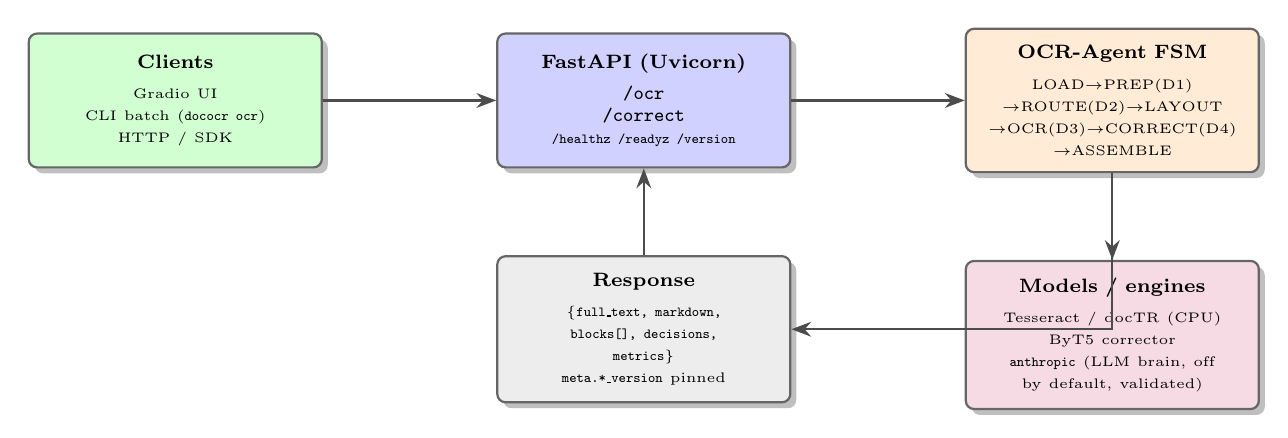
\begin{tikzpicture}[
  node distance=1.0cm and 2.2cm,
  box/.style={rectangle, draw=black!60, rounded corners=3pt, thick,
             text width=3.3cm, minimum height=1.7cm, align=center,
             inner sep=6pt, font=\scriptsize, drop shadow},
  clientbox/.style={box, fill=green!18},
  apibox/.style={box, fill=blue!18},
  agentbox/.style={box, fill=orange!16},
  modelbox/.style={box, fill=purple!14},
  arrow/.style={-{Stealth[length=2.5mm]}, thick, color=black!70}
]

\node[clientbox] (client) {%
  \textbf{Clients}\\[3pt]
  {\tiny Gradio UI}\\
  {\tiny CLI batch (\texttt{dococr ocr})}\\
  {\tiny HTTP / SDK}
};
\node[apibox, right=of client] (api) {%
  \textbf{FastAPI (Uvicorn)}\\[3pt]
  \texttt{/ocr}\\ \texttt{/correct}\\
  {\tiny \texttt{/healthz} \texttt{/readyz} \texttt{/version}}
};
\node[agentbox, right=of api] (agent) {%
  \textbf{OCR-Agent FSM}\\[3pt]
  {\tiny LOAD$\rightarrow$PREP(D1)}\\
  {\tiny $\rightarrow$ROUTE(D2)$\rightarrow$LAYOUT}\\
  {\tiny $\rightarrow$OCR(D3)$\rightarrow$CORRECT(D4)}\\
  {\tiny $\rightarrow$ASSEMBLE}
};
\node[modelbox, below=1.1cm of agent] (models) {%
  \textbf{Models / engines}\\[3pt]
  {\tiny Tesseract / docTR (CPU)}\\
  {\tiny ByT5 corrector}\\
  {\tiny \texttt{anthropic} (LLM brain, off by default, validated)}
};
\node[box, fill=gray!14, below=1.1cm of api, text width=3.3cm] (out) {%
  \textbf{Response}\\[3pt]
  {\tiny \texttt{\{full\_text, markdown,}}\\
  {\tiny \texttt{blocks[], decisions,}}\\
  {\tiny \texttt{metrics\}}}\\
  {\tiny \texttt{meta.*\_version} pinned}
};

\draw[arrow] (client) -- (api);
\draw[arrow] (api) -- (agent);
\draw[arrow] (agent) -- (models);
\draw[arrow] (agent.south) |- (out.east);
\draw[arrow] (out) -- (api);

\end{tikzpicture}%
}
\caption{Deployment architecture. Clients (Gradio / CLI / HTTP) hit one FastAPI service that drives the deterministic OCR-agent FSM; the same backend functions are imported by the Gradio UI (no duplication). Weights are pinned by HF commit SHA and surfaced in \texttt{meta.*\_version} on every response. The LLM brain is off by default, so the default deployment makes \emph{zero} paid API calls and runs on CPU.}
\label{fig:arch}
\end{figure}

\subsection{Response Object and Endpoints}

The \texttt{/ocr} response is lossless and traceable: \texttt{markdown} is the human view, \texttt{blocks[]} the machine view, and every block carries \texttt{type}, \texttt{bbox}, \texttt{text}, \texttt{reading\_index}, OCR confidence, and \texttt{needs\_review}. \texttt{decisions} is the agent audit trail (which of D1--D4 fired). \texttt{meta} pins \texttt{model\_version}, \texttt{pipeline\_version}, and \texttt{engine} independently.

\begin{lstlisting}[basicstyle=\ttfamily\footnotesize]
{ "full_text": "Plain reading-order text of the whole document",
  "markdown":  "## Heading\n\nParagraph text\n\n- list item\n- list item",
  "blocks": [
    { "type": "paragraph", "bbox": [x0,y0,x1,y1], "text": "the results were significant",
      "reading_index": 1, "ocr_conf": 88.0, "needs_review": false } ],
  "decisions": [ { "point": "D2", "choice": "born_digital_skip_ocr" } ],
  "metrics": { },
  "meta": { "model_version": "byt5-postocr@<rev>", "pipeline_version": "ocr-agent@<rev>",
            "engine": "tesseract" } }
\end{lstlisting}

\subsection{Docker, Latency, and Scalability}

The container is built on \texttt{python:3.11-slim} with the native OCR dependencies (\texttt{tesseract-ocr}, \texttt{tesseract-ocr-eng}, \texttt{poppler-utils}, \texttt{libgl1}) installed, since the OCR front-end needs binaries that are not pip-installable; HF weights are pre-downloaded at build so cold start is not a first-request stall.

\begin{table}[H]
\centering
\caption{Latency by path (scanned A4 @300 DPI, CPU default)}
\begin{tabular}{ll}
\toprule
\textbf{Path} & \textbf{Typical latency} \\
\midrule
Born-digital page (D2 skips OCR) & $\sim$\textbf{200\,ms} end-to-end \\
Scanned OCR (dominant cost) & $\sim$0.6--1.2\,s / region \\
Post-OCR correction (small model) & $\sim$80\,ms / region \\
LLM brain (flagged regions only, if enabled) & $\sim$0.8--2\,s \\
\bottomrule
\end{tabular}
\end{table}

The single biggest lever is \textbf{D2}: born-digital pages skip OCR \emph{and} correction. Scalability uses two parallelism axes -- \textbf{page parallelism} (PDFs fan pages across a process pool / queue workers) and \textbf{region parallelism} (regions OCR'd concurrently; correction batched across regions in one model forward pass) -- with GPU batching when present and a CPU-able default for stateless horizontal replicas.

\subsection{Model Versioning}

A model registry (\texttt{models/model\_registry.py}) records each trained corrector with a \texttt{model\_meta.json} + a \texttt{latest} pointer, addressed as \texttt{repo@revision}; pretrained components are pinned by HF commit SHA (not \texttt{main}); D1--D4 thresholds live in a versioned \texttt{config.yaml} so a threshold change is a traceable release. \texttt{GET /version} surfaces the active metadata.

% ============================================================
\section{Agentic AI Component}
% ============================================================

\subsection{Why an Agent}

The intelligence of the system lives in a \textbf{deterministic finite-state machine (FSM)} whose every transition is decided by an explicit rule on measurable signals (DPI, text-layer presence, OCR confidence, edit distance). A single \texttt{JobState} blackboard (\texttt{agent/state.py}) is threaded through every tool and decision, recording \texttt{decisions[]}, \texttt{traces[]} (\texttt{ToolTrace}), and the per-region results -- which makes every run auditable and reproducible via \texttt{manifest.json}. The states are:
\[
\texttt{LOAD} \rightarrow \texttt{PREPROCESS} \rightarrow \texttt{ROUTE} \rightarrow \texttt{LAYOUT} \rightarrow \texttt{OCR} \rightarrow \texttt{CORRECT} \rightarrow \texttt{ASSEMBLE} \rightarrow \texttt{DONE}
\]
(plus a \texttt{FLAG} sink for low-confidence regions). The pipeline is fixed; the ``intelligence'' is the four decision points \textbf{D1--D4}, each with explicit inputs, thresholds, branches, and a safe fallback. (D1--D4 are the four mandatory decision points; together with the D3 human-review \texttt{FLAG} branch and the optional LLM-brain consult, the agent exposes well over five distinct decision behaviours.)

\subsection{The Decision Pipeline}

\begin{figure}[H]
\centering
\resizebox{\linewidth}{!}{%
\begin{tikzpicture}[
  node distance=0.32cm,
  step/.style={rectangle, draw=black!60, rounded corners=2pt, thick,
              text width=13.5cm, inner sep=5pt, minimum height=0.7cm,
              align=center, font=\footnotesize},
  load/.style={step, fill=gray!15},
  dec/.style={step, fill=red!12},
  lay/.style={step, fill=blue!15},
  mod/.style={step, fill=purple!15},
  asm/.style={step, fill=green!15},
  arrow/.style={-{Stealth[length=2mm]}, thick}
]

\node[load] (i) {\textbf{LOAD} (\textit{tool} \texttt{tool\_ingest}): PyMuPDF opens PDF $\rightarrow$ per-page raster image + (PDF) embedded text layer};
\node[dec, below=of i] (d2) {\textbf{D2 -- Route} (\textit{decision}): text layer coverage $\ge$0.80 and $\ge$200 chars? $\rightarrow$ \texttt{born-digital} (\textbf{skip OCR}) else \texttt{scanned}};
\node[dec, below=of d2] (d1) {\textbf{D1 -- Preprocess} (\textit{decision}, scanned only): quality = blur (Laplacian) + ink ratio + contrast $\rightarrow$ \texttt{ok} / \texttt{reprocess} / \texttt{degraded} (lowers D3 bar)};
\node[lay, below=of d1] (lay) {\textbf{LAYOUT} (\textit{tool} \texttt{tool\_layout}): detect regions + type them; \textbf{XY-cut} reading order (2-column aware) $\rightarrow$ \texttt{reading\_index}};
\node[dec, below=of lay] (d3) {\textbf{D3 -- OCR-confidence gate} (\textit{decision}, per region): per-region confidence $<$\,\textbf{0.55} $\rightarrow$ \textbf{FLAG} for human review (kept, \texttt{needs\_review=true})};
\node[mod, below=of d3] (corr) {\textbf{CORRECT} (\textit{tool} \texttt{tool\_correct}): ByT5 \texttt{"correct: <region>"} candidate per region (trained ML core)};
\node[dec, below=of corr] (d4) {\textbf{D4 -- Correction acceptance} (\textit{decision}, per region): accept \emph{iff} edit ratio $\le$\,\textbf{0.35} AND confident; else \textbf{keep raw OCR} (+ optional LLM brain, re-validated)};
\node[asm, below=of d4] (asm) {\textbf{ASSEMBLE} (\textit{tool} \texttt{tool\_assemble}): emit in reading order $\rightarrow$ Markdown + JSON \texttt{blocks[]} + plain text + \texttt{manifest.json}};

\foreach \a/\b in {i/d2, d2/d1, d1/lay, lay/d3, d3/corr, corr/d4, d4/asm}
  \draw[arrow] (\a) -- (\b);

\end{tikzpicture}%
}
\caption{The deterministic OCR-agent FSM with its four decision points. \texttt{tool\_layout} is the composite step running preprocess (D1) + OCR (D3) + reading-order (XY-cut) + block classification, which is what makes the system \emph{document-level}.}
\label{fig:agent}
\end{figure}

\begin{table}[H]
\centering
\caption{The four decision points (signals, deterministic rule, LLM-eligibility)}
\small
\begin{tabularx}{\linewidth}{@{} l l L c @{}}
\toprule
\textbf{DP} & \textbf{State} & \textbf{Deterministic rule} & \textbf{LLM?} \\
\midrule
\textbf{D1} & PREPROCESS & quality(blur, ink, contrast) $\rightarrow$ \texttt{ok} / \texttt{reprocess} / \texttt{degraded}; degraded lowers the D3 bar and forces flag-on-fail & opt.\ (validated) \\
\textbf{D2} & ROUTE & text layer present \& coverage $\ge$0.80 \& chars $\ge$200 $\rightarrow$ born-digital (skip OCR \& layout-from-pixels); else scanned & no \\
\textbf{D3} & OCR (per region) & conf $<$ 0.55 $\rightarrow$ FLAG for human review (kept, \texttt{needs\_review}); thresholds drop on \texttt{degraded} pages & no \\
\textbf{D4} & CORRECT (per region) & accept \emph{iff} edit ratio $\le$ 0.35 AND confident; else keep raw. Flagged/rejected $\rightarrow$ escalate to LLM brain & \textbf{yes} (re-checked) \\
\bottomrule
\end{tabularx}
\end{table}

\textbf{D4 is the safety-critical gate.} It is the single most important safeguard: a corrector that fixes 40\% of regions but breaks 30\% is useless, so a candidate that rewrites more than $\sim$a third of the characters is rejected as untrustworthy and the raw OCR survives. The optional LLM brain (\texttt{anthropic}) is consulted only for \emph{flagged} regions, its proposal is re-validated against the \emph{same} D4 rule, and on any failure (timeout, bad JSON, over budget, no reduction) the FSM falls back to the model output, then to raw. It is \textbf{off by default} $\rightarrow$ zero paid API calls and a CPU-only default run.

\subsection{Worked Example -- a 2-Column Scanned Page}

A scanned PDF page with a title spanning the full width and two text columns below it:

\begin{lstlisting}[basicstyle=\ttfamily\footnotesize]
LOAD       load_page("p12.png") -> source=image, dpi~220, pdf_text_layer=None
ROUTE      has_text_layer -> present=False
           > Decision(D2, text_layer_chars=0, branch=scanned) -> full OCR path
PREPROCESS quality: blur OK, ink normal, contrast slightly low
           > Decision(D1, branch=reprocess) -> light deskew/binarize before OCR
LAYOUT     5 regions: title(order0) | col-1 (order1,2) | col-2 (order3) | figure/caption
           XY-cut detects centre gap -> 2 columns, sorted column-then-top
OCR        title conf 0.91 accept | col1 0.88 accept |
           > Decision(D3, region=col2_para3, conf=0.48, threshold=0.55, branch=review) FLAG
CORRECT    title "lntroductlon" -> "Introduction"  edit_ratio 0.17 <= 0.35
           > Decision(D4, region=title, edit_ratio=0.17, branch=accept)
           col2_para3 (flagged) candidate rewrites >50% chars
           > Decision(D4, region=col2_para3, edit_ratio=0.52, threshold=0.35, branch=keep_raw)
ASSEMBLE   "## Introduction\n\n<col-1 corrected>\n\n<col-2 RAW, flagged for review>"
           blocks[] carry bbox+type+conf+needs_review; manifest.json records all decisions+traces
\end{lstlisting}

\noindent\textbf{Validated offline:} the agent runs end-to-end (ingest $\rightarrow$ layout $\rightarrow$ correct $\rightarrow$ assemble) with \textbf{all four decisions firing}, and a born-digital document produces \textbf{7 typed blocks} with correct Markdown (\texttt{\#\#} headings, \texttt{-} lists) -- with no OCR binary and the LLM off.

% ============================================================
\section{Continual Learning \& Monitoring}
% ============================================================

\subsection{The Feedback Loop}

The known weakness is the \textbf{sim-to-real gap}: synthetic noise may not match the error distribution of the \emph{specific} OCR engine, domain, or scan conditions in production. The cure is to close the loop. The agent already produces two natural sources of supervision:

\begin{table}[H]
\centering
\caption{Production sources of new training data (driven by the decision points)}
\small
\begin{tabularx}{\linewidth}{@{} l c L @{}}
\toprule
\textbf{Source} & \textbf{DP} & \textbf{What it yields} \\
\midrule
Flagged low-confidence regions & D3 & Regions routed to human review (the ``needs-gold'' queue) \\
Rejected corrections (edit ratio $>$ 0.35 or low conf) & D4 & High-value hard cases the model wanted to over-edit \\
Human-corrected gold & review tool & The clean target text for each flagged/rejected region \\
\bottomrule
\end{tabularx}
\end{table}

Each reviewed region becomes one training-ready record in a \textbf{feedback store} with fields \texttt{raw\_ocr} (exactly what the corrector saw), \texttt{corrected\_gold}, \texttt{ocr\_confidence}, \texttt{block\_type}, \texttt{flag\_reason}, \texttt{model\_revision}, \texttt{engine}, \texttt{doc\_domain}, \texttt{language}. These mirror the PleIAs \texttt{text}/\texttt{corrected\_text} columns, so they drop directly into the existing dataset pipeline. Collection is \textbf{privacy-first}: minimal spans, no raw page images, redacted/hashed identifiers.

\subsection{Retraining, Versioning, and Promotion}

Retraining is \textbf{continue-fine-tune} from the current best checkpoint with the same recipe, mixing three streams: (1) real production corrections (highest weight), (2) the real PleIAs slice (anchor general behaviour), (3) fresh synthetic noise (broad coverage). Splits stay leakage-free. Each retrain produces a new \texttt{repo@revision} in the registry. \textbf{Never promote blindly}: a \emph{canary} routes a small fraction of traffic to the new revision; an \emph{A/B} compares it against the incumbent on a frozen \textbf{golden set}; promotion is gated on CER-reduction at least matching the incumbent \emph{and} the safety gate holding (\% degraded stays well below \% improved), with rollback to the previous revision otherwise.

\subsection{Monitoring Metrics}

\texttt{src/dococr/monitoring/drift\_report.py} trends the following over rolling windows:

\begin{table}[H]
\centering
\caption{Monitoring metrics. The first four are continuous from production; the last two require a labelled golden set.}
\small
\begin{tabularx}{\linewidth}{@{} l L @{}}
\toprule
\textbf{Metric} & \textbf{Watch for} \\
\midrule
Flag-rate (\% regions to review at D3) & Sustained increase $\rightarrow$ domain/engine/scan drift \\
Mean region confidence & Sustained decrease $\rightarrow$ input-quality shift \\
Latency (per page / region) & Tail growth $\rightarrow$ profile front-end vs.\ corrector \\
Status mix (auto-accepted / flagged / degraded) & Shift toward flagged/degraded $\rightarrow$ which DP fires more \\
CER-reduction on golden set & Decline vs.\ previous revision $\rightarrow$ block promotion / retrain \\
\% degraded (corrector safety) & Rising / approaching \% improved $\rightarrow$ \textbf{hard fail}, roll back \\
\bottomrule
\end{tabularx}
\end{table}

The D4 edit-budget gate is also a runtime safety net: a degrading model that starts proposing large rewrites gets its corrections auto-rejected, and those regions become new feedback records.

% ============================================================
\section{Data Privacy \& Model Robustness}
% ============================================================

\subsection{Privacy}

A document-level OCR system is, by definition, pointed at whole pages of human documents, which routinely contain PII (names, IDs, addresses, financial data). The posture is data minimization plus local-by-default processing:
\begin{itemize}\setlength\itemsep{0.15em}
  \item \textbf{Minimization \& TTL}: raw images/PDFs are processed transiently, not persisted as a system of record; OCR text/blocks/corrected output live only as long as the request requires; a \textbf{no-retention mode} processes-and-discards.
  \item \textbf{No raw PII in logs}: logs record decisions, timings, and metrics (\texttt{ToolTrace}/\texttt{Decision}/\texttt{manifest.json}) -- \emph{what the agent decided}, not \emph{what the document said}.
  \item \textbf{Local-by-default, no egress}: the ByT5/T5 corrector and Tesseract both run on-device; the optional Anthropic LLM brain is \textbf{off by default}, so the full pipeline can run \textbf{air-gapped} with zero document data leaving the machine.
  \item \textbf{Rights / consent}: the training data avoids the problem entirely -- a synthetic generator over clean English plus the \textbf{CC0-1.0} PleIAs corpus, so no sensitive real documents are scraped.
\end{itemize}

\subsection{Robustness}

OCR input is adversarial by default. Robustness is treated as a \emph{measured} property:
\begin{itemize}\setlength\itemsep{0.15em}
  \item \textbf{OOD scans}: D1 quality routing sends poor scans (skew, blur, low contrast) down the \texttt{degraded} path -- flagging rather than over-rejecting.
  \item \textbf{Noise severity}: the robustness sweep (\texttt{analysis/robustness.py}) confirms CER reduction holds across a \emph{range} of \texttt{char\_error\_rate} levels, not just one operating point; byte-level ByT5 is chosen precisely for this regime.
  \item \textbf{Corrector-makes-it-worse (top risk)}: the D4 bounded-edit guard (ratio $\le$ 0.35) + the \%-degraded safety gate jointly enforce \emph{degraded $\ll$ improved}.
  \item \textbf{Graceful degradation everywhere}: a \textbf{stub OCR engine} (empty result) and an \textbf{identity corrector} let the agent and the whole test suite run with no OCR binary and no \texttt{torch}; \texttt{numpy}/PIL fallbacks replace \texttt{cv2}; optional dataset loaders skip gracefully. The worst case is reduced functionality, not an outage.
\end{itemize}

\textbf{Known failure classes} (flagged, not trusted): dense tables, figures/graphics, rotated scans, complex multi-column layouts, and non-English text (the system is English-first by design and data, stated explicitly).

% ============================================================
\section{Project Management}
% ============================================================

This project was completed \textit{individually}; the work is organized as if six roles existed (PM, ML, Data, OCR/vision, Backend/deploy, QA), with the package directory structure acting as the org chart and code contracts replacing meetings.

\begin{table}[H]
\centering
\caption{Project plan -- eight phases, each with a verifiable exit criterion}
\small
\begin{tabularx}{\linewidth}{@{} c l L @{}}
\toprule
\textbf{\#} & \textbf{Phase} & \textbf{Exit criterion (Definition of Done)} \\
\midrule
P1 & Research \& scoping & Verified model/dataset ids fixed; headline metric = CER/WER \% reduction agreed \\
P2 & Synthetic generator + baselines & 60k/4k/4k splits built; identity floor measured (CER 0.088, WER 0.49) \\
P3 & OCR / layout integration & Born-digital doc $\rightarrow$ typed blocks in correct reading order; Markdown + JSON \\
P4 & ByT5 fine-tune & Trained ByT5 reduces CER below identity with degraded $\ll$ improved \\
P5 & Agent & All four decisions fire end-to-end; full audit trace + \texttt{manifest.json} \\
P6 & Deployment & API serves uploads; Docker (tesseract+poppler) builds; HF Space packaged \\
P7 & Evaluation & Headline reduction + robustness sweep + real PleIAs CER reported \\
P8 & Docs \& report & Report + slides generate; submission package complete \\
\bottomrule
\end{tabularx}
\end{table}

\noindent The critical path is \texttt{P1$\rightarrow$P2$\rightarrow$P4$\rightarrow$P5$\rightarrow$P6$\rightarrow$P7$\rightarrow$P8}, with \textbf{P3 (OCR/layout)} able to overlap \textbf{P4 (ByT5 fine-tune)} because the corrector trains on text pairs and does not need the OCR front-end to exist. The longest compute task is the ByT5 fine-tune ($\approx$3--6\,h on one H100). \textbf{Scaling reflection}: the four module-aligned squads (OCR/vision, ML, Data, Platform) synchronize at just two contracts -- the block schema (vision $\rightarrow$ ML) and the API response schema (platform $\rightarrow$ consumers) -- and the existing offline guarantees (stub OCR, identity corrector, fallbacks) become the foundation of CI, where a \textbf{safety-gate regression check} blocks any PR that raises \% degraded.

% ============================================================
\section{Ethics \& Responsible AI}
% ============================================================

Because the system both \emph{transcribes} documents and \emph{rewrites} the transcribed text, it raises two ethical surfaces: privacy/consent over what gets transcribed, and faithfulness over what the corrector changes.

\subsection{Who Benefits, Who Could Be Harmed}

\textbf{Benefits}: archivists/libraries (searchable structured collections), businesses (machine-readable records, cheaper born-digital pages), accessibility users (reading-order-correct text for screen readers), researchers (clean, auditable corpora). \textbf{Harms}: people whose private documents become instantly queryable without consent; anyone relying on a high-stakes document (legal, medical, financial) where the corrector silently ``fixes'' a real but unusual string (a case number, dosage, or account figure) into something more plausible -- a hallucinated correction in such a document is the single most dangerous failure mode.

\subsection{Bias \& Fairness}

The system is \textbf{English-first by design and by data} (synthetic noise over clean English + the single real English PleIAs corpus). A model trained mostly on synthetic noise plus one real English corpus will likely underperform on other languages, scripts, domains, and genres whose error distributions differ. \textbf{Honest disclosure}: do not deploy the corrector on non-English, non-Latin, or specialized-domain text without re-measuring CER reduction and the safety gate on that distribution. Equal headline accuracy across all inputs is \emph{not} claimed; the sim-to-real gap is mitigated by mixing real PleIAs data and reporting real-corpus CER alongside synthetic CER.

\subsection{Mitigating the Meaning-Altering Risk}

The core responsible-AI concern is the generative corrector hallucinating. Mitigations, in layers:
\begin{enumerate}\setlength\itemsep{0.1em}
  \item \textbf{Bounded edit budget (D4)}: accept only if \texttt{edit\_ratio $\le$ 0.35} and confident -- a corrector structurally cannot rewrite a region away.
  \item \textbf{The \%-degraded safety gate}: require \texttt{degraded $\ll$ improved}; a corrector that fixes 40\% but breaks 30\% is a failure, not a success.
  \item \textbf{Human-review gate}: low-confidence regions (D3 $<$ 0.55) and degraded pages (D1) are routed to people, not auto-accepted.
  \item \textbf{Identity baseline kept honest}: any version that does not beat identity (CER 0.088) is rejected.
\end{enumerate}
The optional LLM brain is off by default and, when enabled, only assists flagged regions and is re-validated against the same rule -- it never gets an unbounded license to rewrite.

\subsection{Misuse and Safeguards}

Foreseeable misuse includes mass/bulk transcription of private documents and scraping copyrighted material at scale. Safeguards built around the pipeline: rights/consent treated as a precondition; an audit \texttt{manifest.json} making every run accountable; the human-review gate (D3/D1); the D4 edit budget bounding silent alteration; and privacy-minimizing operation (minimal retention, on-prem/no-retention, TTL). These are technical guardrails, not a substitute for the operator's legal responsibility for lawful basis, consent, and copyright -- the system is designed to make those obligations \textbf{visible and auditable}.

% ============================================================
\section{Conclusion \& Future Work}
% ============================================================

\subsection{Summary}

\begin{itemize}\setlength\itemsep{0.15em}
  \item Complete end-to-end system: data $\rightarrow$ training $\rightarrow$ evaluation $\rightarrow$ deployment $\rightarrow$ monitoring, for document image/PDF $\rightarrow$ clean, structured, reading-order-correct text (Markdown + JSON blocks + plain text).
  \item Trained differentiator: a byte-level \texttt{google/byt5-small} post-OCR corrector that lowers CER/WER on top of \emph{any} OCR engine, judged by error \emph{reduction} against an identity floor (CER 0.088, WER 0.49) and a per-example safety gate (\% degraded $\ll$ \% improved).
  \item A deterministic four-decision agent (D1 preprocess, D2 born-digital routing, D3 confidence gate, D4 correction acceptance) with a full audit trace, validated offline (all four decisions fire; a born-digital doc yields 7 typed blocks with correct Markdown).
  \item Deployable as a FastAPI REST API + Gradio UI + CLI + Docker + HF Space packaging, with a one-button Colab H100 autopilot that trains, evaluates, self-grades, and auto-generates the report/slides.
\end{itemize}

\subsection{Future Work}

\begin{enumerate}\setlength\itemsep{0.1em}
  \item \textbf{Close the sim-to-real gap}: harvest real \texttt{(raw OCR, corrected)} pairs from the D3/D4 flows and continue-fine-tune per engine/domain.
  \item \textbf{Stronger structure}: learned reading order (Surya / PP-StructureV3) and Table-Transformer cell structure as upgrades behind the same engine interface.
  \item \textbf{Larger corrector}: a base/large ByT5 (or a domain-adapted variant) to push CER reduction further where latency budget allows.
  \item \textbf{More languages}: expand training data per language before claiming multilingual support, with out-of-scope languages routed to review.
  \item \textbf{Observability}: a drift dashboard reading from \texttt{drift\_report.py} with alerting on flag-rate / \% degraded, plus canary A/B for new model revisions.
\end{enumerate}

% ============================================================
\newpage
\begin{thebibliography}{9}

\bibitem{byt5} Xue, L., Barua, A., Constant, N., et al. (2022). ByT5: Towards a Token-Free Future with Pre-trained Byte-to-Byte Models. \textit{TACL}; arXiv:2105.13626.

\bibitem{t5} Raffel, C., et al. (2020). Exploring the Limits of Transfer Learning with a Unified Text-to-Text Transformer (T5). \textit{JMLR 21}.

\bibitem{pleias} PleIAs. \textit{Post-OCR-Correction} dataset (config \texttt{english}, CC0-1.0). Hugging Face Datasets. \url{https://huggingface.co/datasets/PleIAs/Post-OCR-Correction}

\bibitem{icdar} Rigaud, C., Doucet, A., Coustaty, M., \& Moreux, J.-P. (2019). ICDAR 2019 Competition on Post-OCR Text Correction. \textit{ICDAR 2019}.

\bibitem{jiwer} Vaessen, N., et al. \textit{jiwer}: CER/WER via RapidFuzz edit distance. \url{https://github.com/jitsi/jiwer}

\bibitem{symspell} Garbe, W. \textit{SymSpell} / \texttt{symspellpy}: Symmetric Delete spelling correction. \url{https://github.com/wolfgarbe/SymSpell}

\bibitem{tesseract} Smith, R. (2007). An Overview of the Tesseract OCR Engine. \textit{ICDAR 2007}.

\bibitem{doctr} Mindee. \textit{docTR}: Document Text Recognition (DBNet + CRNN/ViTSTR). \url{https://github.com/mindee/doctr}

\bibitem{tabletransformer} Smock, B., Pesala, R., \& Abraham, R. (2022). PubTables-1M / Table Transformer. \textit{CVPR 2022}; arXiv:2110.00061.

\bibitem{huggingface} Wolf, T., et al. (2020). Transformers: State-of-the-Art Natural Language Processing. \textit{EMNLP 2020}.

\bibitem{fastapi} Ram\'irez, S. (2018). FastAPI. \url{https://fastapi.tiangolo.com/}

\end{thebibliography}

\end{document}
